
\chapter{TINJAUAN PUSTAKA}
\label{chap:tinjauanpustaka}

% Ubah bagian-bagian berikut dengan isi dari tinjauan pustaka

Pada penelitian sebelumnya berjudul "Language Models for Human-Robot Interaction" dengan tujuan untuk menunjukkan potensi dan batasan dari model bahasa besar dalam konteks interaksi manusia-robot secara langsung \parencite{inproceedings}. Dalam penelitian ini, model bahasa besar OpenAI GPT-3 berhasil diintegrasikan dengan robot Pepper dan Nao untuk menciptakan sistem dialog verbal terbuka. Saat pengujian, model yang digunakan adalah GPT-3 Davinci, dan hasil implementasi ini disajikan memberikan kesempatan untuk partisipan manusia untuk terlibat dalam percakapan terbuka dengan robot Pepper dan Nao, memungkinkan mereka untuk memahami batasan dari model bahasa besar dalam konteks interaksi manusia-robot. Meskipun berhasil di tahap pengujian, perlu dicatat bahwa robot menggunakan model yang belum terintegrasi sepenuhnya dengan robot dan tidak memiliki informasi umum mengenai keadaan robot ataupun lingkungan sekitarnya.

\section{Interaksi Robot-Manusia}
Interaksi Manusia-Robot (HRI) adalah disiplin ilmu yang mempelajari tentang dinamika interaksi antara manusia dan robot \parencite{VASCONEZ201935}. Disiplin ini memfokuskan pada pemahaman, perancangan, dan evaluasi cara manusia dan robot berinteraksi di berbagai konteks dengan manusia. Tujuan utamanya adalah untuk membuat interaksi antara manusia dan robot semakin lancar dan terasa alami, sehingga mengurangi waktu yang dibutuhkan bagi pengguna untuk beradaptasi. Dengan perkembangan teknologi yang semakin maju dan penetrasi robot yang semakin luas dalam berbagai aspek kehidupan manusia, sangat penting untuk memberikan prioritas pada pengalaman pengguna dan memastikan bahwa setiap interaksi tersebut mudah dipahami, efisien, dan, yang terpenting, berfokus pada kebutuhan manusia \parencite{chikwendu2023human}. Dalam interaksi robot-manusia, sangat penting untuk menganalisis dan mengoptimalkan aspek-aspek seperti antarmuka pengguna, perilaku robot, dan dampak yang mungkin timbul selama interaksi tersebut dengan tujuan menciptakan interaksi yang efektif, intuitif, dan mendukung kerjasama harmonis antara manusia dan robot dalam berbagai konteks. Pemahaman bahasa manusia oleh robot, baik melalui pemrosesan bahasa alami maupun pengenalan suara, memungkinkan interaksi yang lebih kompleks dan alami. 


Di sektor industri, interaksi robot-manusia telah menciptakan lingkungan kerja yang dinamis. Robot kolaboratif adalah jenis robot yang dapat bekerja bersama manusia dengan aman, menghadirkan peluang untuk meningkatkan produktivitas dan efisiensi. Sementara itu, di bidang layanan dan kesehatan, robot memberikan dukungan dalam pemantauan kesehatan dan terapi, membawa dampak positif dalam pelayanan dan kesejahteraan manusia.

\section{Robot \textit{Service}}
Robot \textit{Service} adalah robot yang dirancang untuk memberikan layanan kepada manusia \parencite{electronics10212658}. Robot service memiliki di berbagai bidang, seperti rumah tangga dan komersial. Dalam mendukung interaksi dengan manusia, Robot \textit{service} dapat menerapkan berbagai metode komunikasi, termasuk melalui ucapan, tindakan, dan antarmuka yang dirancang intuitif. Sensor-sensor seperti sensor suara, kamera, dan sensor gerak membekali Robot \textit{service} dengan kemampuan responsif terhadap perubahan lingkungan sekitar, menciptakan pengalaman interaksi yang dinamis.

Aplikasi yang luas mencakup berbagai sektor, seperti layanan pelanggan, di mana robot service dapat memberikan informasi, bantuan, atau menerima pesanan. Sebagai asisten pribadi, kemampuannya membantu dalam manajemen jadwal dan memberikan informasi cuaca memperluas perannya di kehidupan sehari-hari. Di sektor kesehatan, robot \textit{service} dapat memberikan dukungan atau mengingatkan jadwal obat, sementara di bidang pendidikan, menjadi penyajian materi pembelajaran yang interaktif. Robot \textit{service} dapat membantu dalam perkembangan teknologi untuk memperbaiki kualitas layanan dan membentuk interaksi manusia dengan mesin menjadi lebih responsif dan dinamis.

\section{Dobot Magician}
\label{sec:dobot-magician}

% Contoh input gambar
\begin{figure}[H]
  \centering

  % Ubah dengan nama file gambar dan ukuran yang akan digunakan
  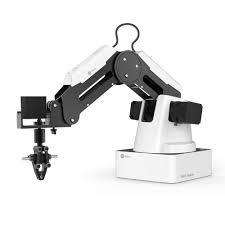
\includegraphics[scale=0.8]{gambar/dobot.jpeg}

  % Ubah dengan keterangan gambar yang diinginkan
  \caption{Dobot Magician \parencite{dobotus}.}
  \label{fig:roketluarangkasa}
\end{figure}

Dobot Magician adalah robot lengan kolaboratif yang memiliki 4 poros. Robot ini memiliki tingkat akurasi yang tinggi, yakni sekitar 0,2 mm, dan menggunakan chip industri STM32 sebagai pengontrolnya. Untuk mengontrol robot ini, tersedia \emph{API} dalam bahasa pemrogaman \emph{Python} yang dapat digunakan oleh pengembang untuk mengntrol robot. Robot ini juga mempunyai Aplikasi Dobot Lab yang menawarkan fitur pengontrol berbasis \emph{Graphical User Interface} untuk mempermudah pengguna tanpa latar belakang dalam pemrogaman untuk mengontrol robot. Robot ini juga memiliki berbagai macam pilihan \emph{end effector} yang dapat digunakan untuk mengatur fungsionaliitas robot. \emph{End effector} yang tersedia meliputi pencapit (\emph{claw}) untuk menjepit objek, penghisap (\emph{suction cup}) yang dapat digunakan untuk menyedot objek, pena untuk melakukan penulisan atau penggambaran, dan ada juga aksesoris yang dapat digunakan untuk melakukan pencetakan 3d. Untuk aksesoris yang digunakan diluar \emph{end effector} terdapat aksesori citra \emph{vision} yang dapat digunakan untuk pengolahan citra dan juga \emph{conveyor belt} untuk memindahkan barang.

\begin{figure}[H]
  \centering

  % Ubah dengan nama file gambar dan ukuran yang akan digunakan
  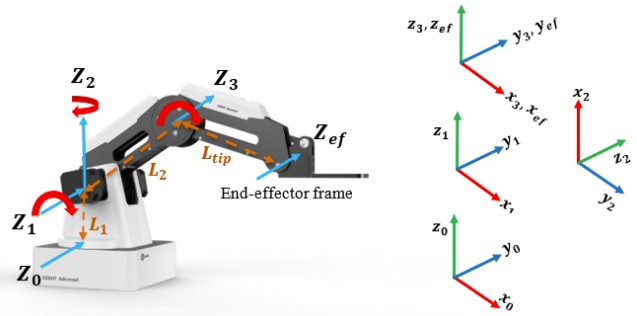
\includegraphics[scale=0.9]{gambar/kinem.jpg}

  % Ubah dengan keterangan gambar yang diinginkan
  \caption{Kinematika \parencite{inproceedings}.}
  \label{fig:roketluarangkasa}
\end{figure}


  \begin{table}[h]
    \centering
    \begin{tabular}{|c|c|c|c|c|}
        \hline
        Link & Link Twist & Link Length & Link Offset & Joint Angle \\
        $i$ & $\alpha_{i-1}$ & $a_{i-1}$ & $d_i$ & $\theta_i$ \\
        \hline
        1 & 0 & 0 & $d$ & $\theta_1$ \\
        2 & $\frac{\pi}{2}$ & 0 & 0 & $\theta_2$ \\
        3 & 0 & $a_1$ & 0 & $\theta_3$ \\
        4 & 0 & $a_2$ & 0 & $\theta_4$ \\
        \hline
    \end{tabular}
    \caption{Denavit-Hartenberg Parameters}
    \label{tab:dh-parameters}
\end{table}

Berikut ini adalah kinematika dan parameter Denavit-Hartenberg robot lengan Dobot Magician. Robot ini mempunyai empat \textit{joint}. \textit{Joint} pertama terletak di \textit{base}, \textit{joint} kedua terletak di lengan bagian belakang, \textit{joint} ketiga terletak di lengan bagian depan, dan \textit{joint} keempat terletak dekat \textit{end effector}.


\section{Model Bahasa Besar}

Model bahasa besar adalah model yang dirancang untuk dapat memahami dan menghasilkan teks \parencite{2023arXiv230706435}. Model ini menggunakan teknik \textit{deep learning} dan pemrosesan bahasa alami untuk mengenali pola dalam teks, dan kemudian menggunakan pola tersebut untuk menghasilkan teks baru. Untuk melakukan training dalam model bahasa besar, diperlukan data teks dengan jumlah sangat besar dan kualitasnya akan mempengaruhi performa model bahasa \parencite{liu2024understanding}.

Perkembangan model bahasa besar tidak lepas dengan perkembangan arsitektur transformer. Arsitektur transformer adalah salah satu jenis arsitektur dalam \textit{neural network} yang populer digunakan untuk pemrosesan teks. Model ini menggunakan mekanisme \textit{attention} untuk menangkap hubungan jarak jauh antara kata-kata, sehingga memungkinkan model untuk memahami konteks teks. Pada arsitektur transformer, \textit{attention} adalah proses yang memungkinkan model untuk memfokuskan pada kata-kata tertentu dalam teks \parencite{vaswani2023attention}. Proses ini dilakukan dengan menghitung skor \textit{attention} untuk setiap kata dalam teks. Skor \textit{attention} ini kemudian digunakan untuk menentukan seberapa besar pengaruh kata tersebut terhadap kata yang sedang diproses.

\begin{figure}[H]
  \centering

  % Ubah dengan nama file gambar dan ukuran yang akan digunakan
  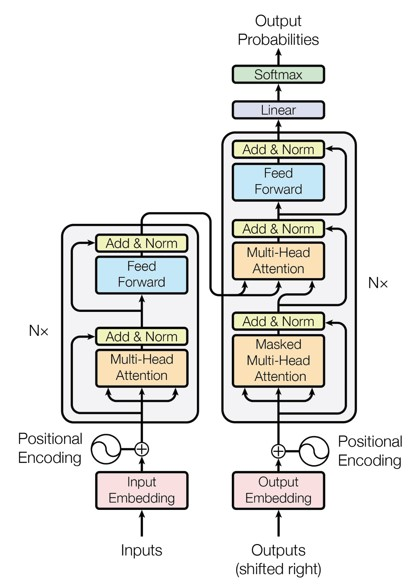
\includegraphics[scale=0.8]{gambar/transformer.jpg}

  % Ubah dengan keterangan gambar yang diinginkan
  \caption{Arsitektur Transformer \parencite{vaswani2023attention}.}
\end{figure}

Model GPT \textit{Generative Pre-training Transformer} dan PaLM \textit{Pathways Language Model} adalah dua model bahasa besar populer yang dikembangkan oleh OpenAI dan Google. Kedua model ini menggunakan mekanisme \textit{attention} untuk menangkap hubungan jarak jauh antara kata-kata, sehingga memungkinkan model bahasa besar untuk memahami konteks teks.

\subsection{Gemma}

% Contoh input gambar
\begin{figure}[H]
  \centering

  % Ubah dengan nama file gambar dan ukuran yang akan digunakan
  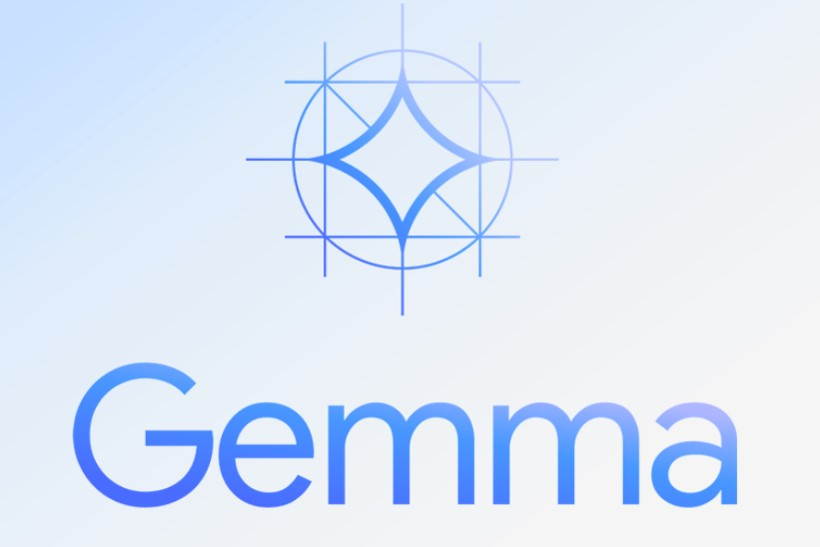
\includegraphics[scale=0.5]{gambar/gemma.jpg}

  % Ubah dengan keterangan gambar yang diinginkan
  \caption{Logo Gemma \parencite{gemma}.}
  \label{fig:roketluarangkasa}
\end{figure}

Gemma adalah sebuah model bahasa besar yang bersifat \emph{open source} dan ringan yang dikembangkan oleh Google DeepMind. Model-model ini dirancang untuk memahami dan menghasilkan teks dengan kemampuan yang serupa dengan manusia, serta dapat digunakan untuk berbagai aplikasi dalam bidang pemrosesan bahasa alami, seperti memahami teks, menghasilkan teks, dan penerjemahan. Gemma merupakan model teks ke teks yang berarti mempunyai input teks dan menghasilkan output teks.

\begin{figure}[H]
  \centering

  % Ubah dengan nama file gambar dan ukuran yang akan digunakan
  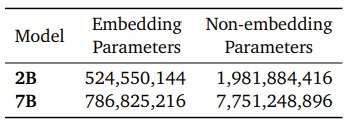
\includegraphics[scale=1]{gambar/param_gemma.jpg}

  % Ubah dengan keterangan gambar yang diinginkan
  \caption{Ukuran Parameter Gemma \parencite{gemma}.}
\end{figure}

\begin{figure}[H]
  \centering

  % Ubah dengan nama file gambar dan ukuran yang akan digunakan
  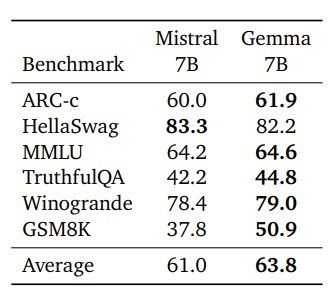
\includegraphics[scale=1]{gambar/gemma-bench.jpg}

  % Ubah dengan keterangan gambar yang diinginkan
  \caption{Benchmark Gemma 7B dan Mistral 7B \parencite{gemma}.}
\end{figure}

Gemma hadir dengan dua jenis ukuran parameter, 2b dan 7b. Jenis ukuran ini merepresentasikan jumlah paramater yang dilatih dalam model bahasa. Model Gemma 7b memiliki arsitektur yang lebih kompleks, cocok digunakan untuk menangani pemrosesan bahasa yang memerlukan pemahaman konteks yang kompleks dan penanganan tugas NLP yang lebih mendalam. Di sisi lain, Gemma 2b dirancang untuk melakukan pemrosesan bahasa pada perangkat dengan sumber daya komputasi yang lebih kecil, memastikan kinerja yang optimal dalam lingkungan yang memiliki keterbatasan sumber daya komputasi. Berdasarkan hasil benchmark, model Gemma memiliki rata - rata performa terbaik dibandingkan model lain dengan ukuran paramater sejenis.

\subsection{\textit{Low Rank Adaptation}}

\textit{Low Rank Adaptation} atau disingkat LoRA merupakan teknik untuk melakukan \textit{fine tuning} yang digunakan model bahasa besar untuk menyesuaikan dengan data spesifik yang baru tanpa harus melatih ulang seluruh model. Teknik ini melibatkan pengurangan dimensi dari representasi internal model, yang dapat dilakukan dengan menggunakan metode faktorisasi matriks (\textit{Low Rank Matrix}). Dengan mengurangi kompleksitas model, low rank adaptation memungkinkan penyesuaian yang cepat dan efisien terhadap data baru, sambil tetap mempertahankan sebagian besar pengetahuan yang telah diperoleh oleh model asli.

\begin{figure}[H]
  \centering

  % Ubah dengan nama file gambar dan ukuran yang akan digunakan
  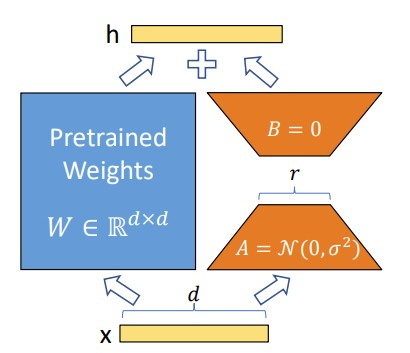
\includegraphics[scale=0.8]{gambar/lora.jpg}

  % Ubah dengan keterangan gambar yang diinginkan
  \caption{Mekanisme kerja LoRA \parencite{gemma}.}
\end{figure}

Dengan menggunakan proses ini, memungkinkan model untuk memperoleh pemahaman yang lebih mendalam terhadap data spesifik tertentu dengan menghilangkan komponen yang kurang relevan atau umum dari representasi internalnya. Kemudian, model yang telah disesuaikan dapat digunakan untuk tugas-tugas khusus dalam domain tersebut dengan kinerja yang lebih baik daripada model yang belum disesuaikan. Keunggulan utama LoRA terletak pada efisiensi dalam penyesuaian model: sebuah model yang telah dilatih sebelumnya dapat dibagi dan digunakan untuk membangun banyak modul LoRA kecil untuk tugas-tugas yang berbeda. 


\section{Multimodalitas}
\label{sec:gravitasi}

Sistem interaksi manusia-komputer multimodal terdiri dari penggunaan berbagai saluran input dan output \parencite{jia2020multimodal}. Pendekatan multimodal ini mengintegrasikan beberapa mode komunikasi, seperti teks, suara, gambar, dan gerakan, untuk menciptakan pengalaman interaktif yang lebih kaya. Dengan memanfaatkan keberagaman saluran ini, sistem dapat mengoptimalkan cara pengguna berinteraksi dengan perangkat komputer. Pengguna dapat memberikan input melalui berbagai cara, seperti mengetik, berbicara, atau menggunakan gerakan tubuh, sedangkan output dapat disampaikan melalui teks, suara, visual, atau kombinasi dari semuanya. Pendekatan multimodal bertujuan untuk meningkatkan aksesibilitas, efisiensi, dan pengalaman pengguna dalam berbagai konteks, memungkinkan interaksi yang lebih intuitif dan menyeluruh antara manusia dan sistem komputer.

% Contoh input gambar
\begin{figure}[H]
  \centering

  % Ubah dengan nama file gambar dan ukuran yang akan digunakan
  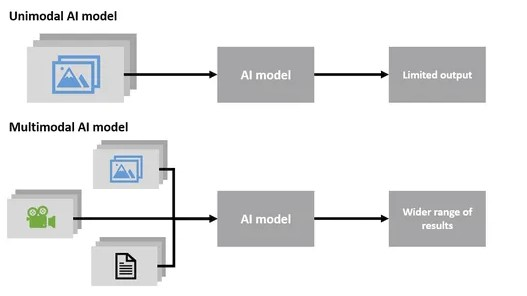
\includegraphics[scale=0.8]{gambar/konsep_mul.jpg}

  % Ubah dengan keterangan gambar yang diinginkan
  \caption{Konsep Multimodal \parencite{dobotus}.}
\end{figure}


Penerapan multimodalitas dapat ditemukan dalam berbagai aplikasi, seperti asisten pintar, perangkat seluler, dan sistem interaktif. Misalnya, dalam asisten pintar, pengguna dapat berinteraksi dengan menggunakan kombinasi suara dan teks untuk memberikan perintah atau mendapatkan informasi. Pada perangkat seluler, layar sentuh, suara, dan gerakan dapat digunakan bersamaan untuk memberikan pengalaman pengguna yang lebih interaktif. Pada perangkat pintar rumah, sistem multimodal dapat mengukur suhu ruangan dan jumlah orang di dalam ruangan untuk mengatur suhu pendingin ruangan. Sistem multimodal juga membuka peluang untuk meningkatkan aksesibilitas, memungkinkan individu dengan berbagai kebutuhan untuk berinteraksi dengan cara yang paling nyaman. Dengan menggabungkan berbagai modalitas, multimodalitas tidak hanya memperkaya interaksi antara manusia dan teknologi, tetapi juga mendukung pengembangan sistem yang lebih inklusif dan responsif


\section{OpenCV}

\begin{figure}[H]
  \centering

  % Ubah dengan nama file gambar dan ukuran yang akan digunakan
  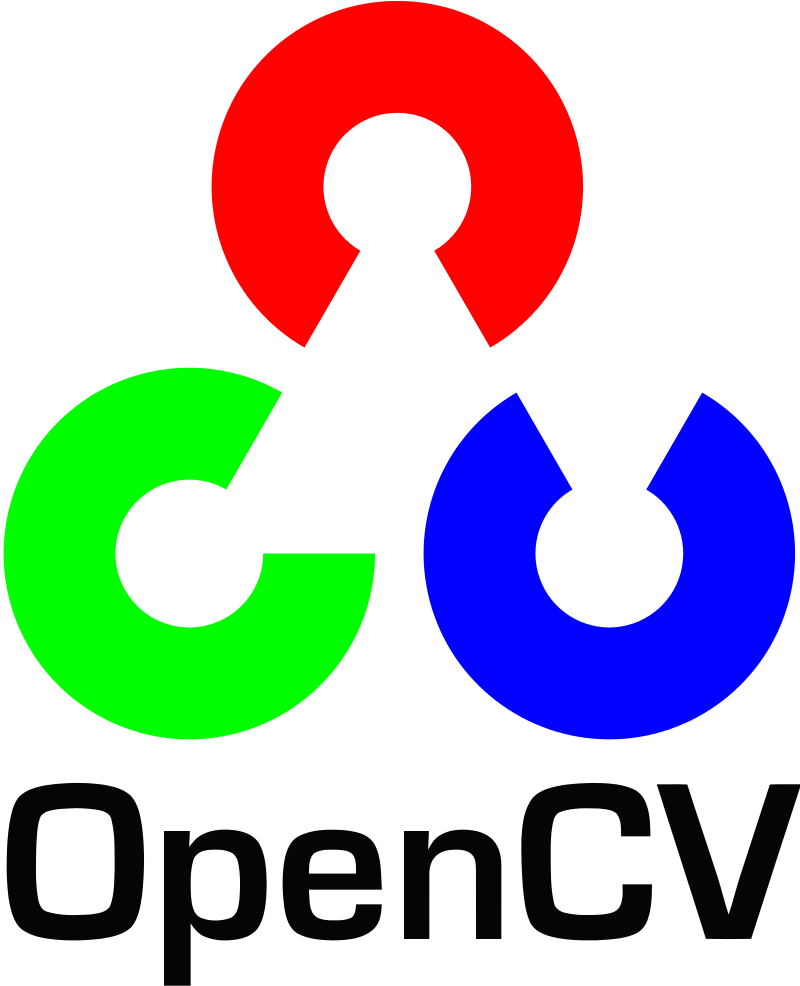
\includegraphics[scale=0.1]{gambar/opencv.png}

  % Ubah dengan keterangan gambar yang diinginkan
  \caption{Logo OpenCV \parencite{opencv_about}.}
\end{figure}

OpenCV \textit{(Open Source Computer Vision Library)} adalah sebuah library bersifat terbuka yang menyediakan berbagai fungsi untuk  melakukan pengolahan citra dan video pada komputer \parencite{opencv_about}. OpenCV telah menjadi salah satu \textit{library} perangkat lunak paling populer dan sangat dipercaya dalam pengolahan citra dan video komputer. Pustaka ini menawarkan beragam alat dan fungsi yang sangat berguna dalam berbagai aplikasi, seperti deteksi objek, pelacakan gerakan, pengenalan pola, dan segmentasi citra.







  

